\section{Results}
Subjects generally performed well at the orientation discrimination task. The mean orientation discrimination threshold across participants was 6.6\textdegree, and behavioral performance was quite stable across runs.

\subsection{Spatial attention increases fMRI response amplitudes}
First, we determined whether directing attention to a spatial location led to stronger overall responses in the visual cortex. Regions of interest consisted of voxels that were significantly activated by the stimulus in all layers of areas V1, V2, and V3 (see Methods). We compared the amplitude of the BOLD response with and without attention, for trials in which a stimulus was presented and those in which no stimulus appeared (see Fig.~\ref{fig:roiresults}). Data were analyzed using a general linear model with area, attention (attended vs. unattended), and stimulus (present vs. absent) as factors (see Methods). We first focused on the effects of attention per se. Attention significantly enhanced the BOLD response at the attended location in areas V1-V3 (effect of attention, F(1, 16) = 43.4, p = 6.36$\cdot10^{-6}$), with a trending increase in attention-based activity for higher-level areas (interaction between attention and area, F(2, 32) = 2.63, p = 0.088). The mean effect sizes (in percent signal change) were 0.41\%, 0.64\% and 0.59\% for V1, V2, and V3 respectively, and slightly stronger to those reported before \cite{Murray2008,Jehee2011}. Next, we investigated whether the effects of attention depended on the presence of a visual stimulus. Specifically, we compared attentional effects between trials in which observers were expecting a stimulus but none was presented, and trials in which the stimulus did appear on the screen. Replicating previous reports \cite{Kastner1999}, the effect of attention in areas V1-V3 was not significantly different in the absence compared to presence of visual stimulation (two-way interaction between and attention and stimulus, F(1, 16) = 0.26, p = 0.585), with no reliable change across areas (three-way interaction between stimulus, attention and area, F(2, 32) = 0.026, p = 0.901). Thus, attending to a spatial location enhances the BOLD response at that location, even in the absence of visual stimulation.
\begin{figure}[!ht]
\centering
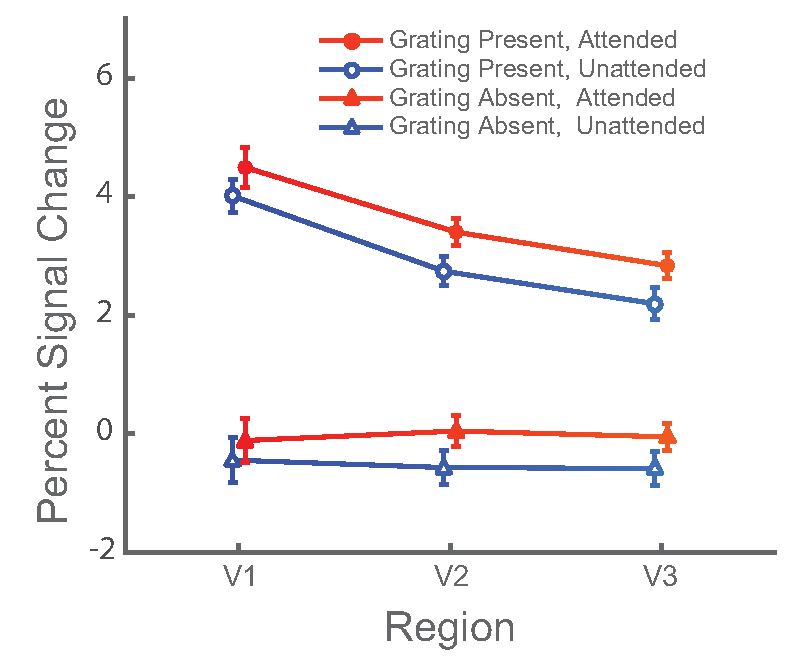
\includegraphics[width=0.8\textwidth, clip=true]{./Chapters/04_Attention/Images/RoiResults}
\caption{Amplitude of the BOLD response for attended and unattended regions in areas V1-V3. Red lines indicate the attended condition, blue the unattended. The top lines (circles) show the response when a grating was presented, the bottom lines (triangles) when no grating was presented, at the attended or unattended location. Response amplitudes were significantly higher for attended than unattended locations and stimuli. Error bars indicate $\pm$1 SEM.}
\label{fig:roiresults}
\end{figure}

\subsection{Spatial attention increases responses across the layers}
Next, we asked whether attention led to changes in the pattern of activity across cortical layers in these areas. We used a spatial general linear model (see methods) to first characterize activity in each of three distinct cortical layers. Data were subsequently analyzed using a temporal general linear model with attention, stimulus, area, and layer as factors (see Methods). Consistent with previous studies \cite{Koopmans2010,Polimeni2010}, we found a general increase in BOLD response from white matter to pial surface (see Fig~\ref{fig:layerresults}, overall effect of layer, F(2, 32) = 12.5, p = 9.85$\cdot10^{-5}$). This increase in BOLD response with decreasing distance to the pial surface was reliably larger in the presence of a stimulus (two-way interaction between layer and stimulus, F(2, 32) = 61.1, p = 1.00$\cdot10^{-11}$), and was significantly different between the three areas (three-way interaction between layer, stimulus, area: F(4, 64) = 3.33, p = 0.015; post hoc analyses revealed a trending larger effect for area V1 compared to V2 (T(16) = 2.11, p = 0.051), and a larger effect for area V2 compared to areas V3 (T(16) = 3.37, p = 0.0039). This tendency of the BOLD response to increase from lower layers to higher layers should be interpreted with caution, however, as blood flows from the gray-white matter boundary towards the pial surface. Hence, any change in BOLD response that arises in layers V-VI will automatically affect the BOLD response in downstream layers. This accumulation of signal may also result in a larger slope of activation through the layers for larger effects with equal laminar activation, thus explaining the greater layer by stimulus interaction in earlier visual regions. In contrast to the layer-specific increase in BOLD signal when presenting a stimulus, we found no significant change in the effects of spatial attention across the layers (two-way interaction between layer and attention, F(2, 32) = 2.33, p = 0.114). This may reflect equal activation of all layers, or a rather shallow slope as a result of low attentional effect. Next, we determined whether the layer-specific increase in BOLD signal with attention was distinct from the observed stimulus-based effects. The attention-based increase in activity was indeed reliably different from stimulus-driven changes in layer response (post hoc comparison between layer by stimulus effect and layer by attention effect; T(16) = 4.94, p = 1.47$\cdot10^{-4}$). However, this effect should be interpreted with caution, as the strength of the layer responses is tightly coupled to the strength of the main effects. In addition, there was no reliable difference between the effects of attention versus stimulus between any of the three layers (three-way interaction between layer, stimulus and attention, F(2, 32) = 1.69, p = 0.200). Control analyses established that these results were not strongly affected by the number of voxels included in the analyses (Supplementary Figures~\ref{fig:layerresults300}-\ref{fig:layerresults900}), nor by the number of layers analyzed (Supplementary Figure~\ref{fig:layerresults4layers}). In addition, these results did not qualitatively change when layer activation profiles were defined using volume interpolation (Supplementary Figure~\ref{fig:layerresultsinterp}). Moreover, combining the anticipation (i.e., time frame prior to when a stimulus could appear, see Figure~\ref{fig:experiment}) and stimulus windows in the analyses did not reliably affect any of these results (Supplementary Figure~\ref{fig:layerresultsplusattention}). Thus, while the overall effects on BOLD activity of both visual stimuli and attention were rather robust and similar to previously reported values for visual cortex \cite{Kastner1999,Jehee2011, Koopmans2010}, no differential pattern of activity was observed between these two processes across the visual cortical layers.
\begin{figure}[!ht]
\centering
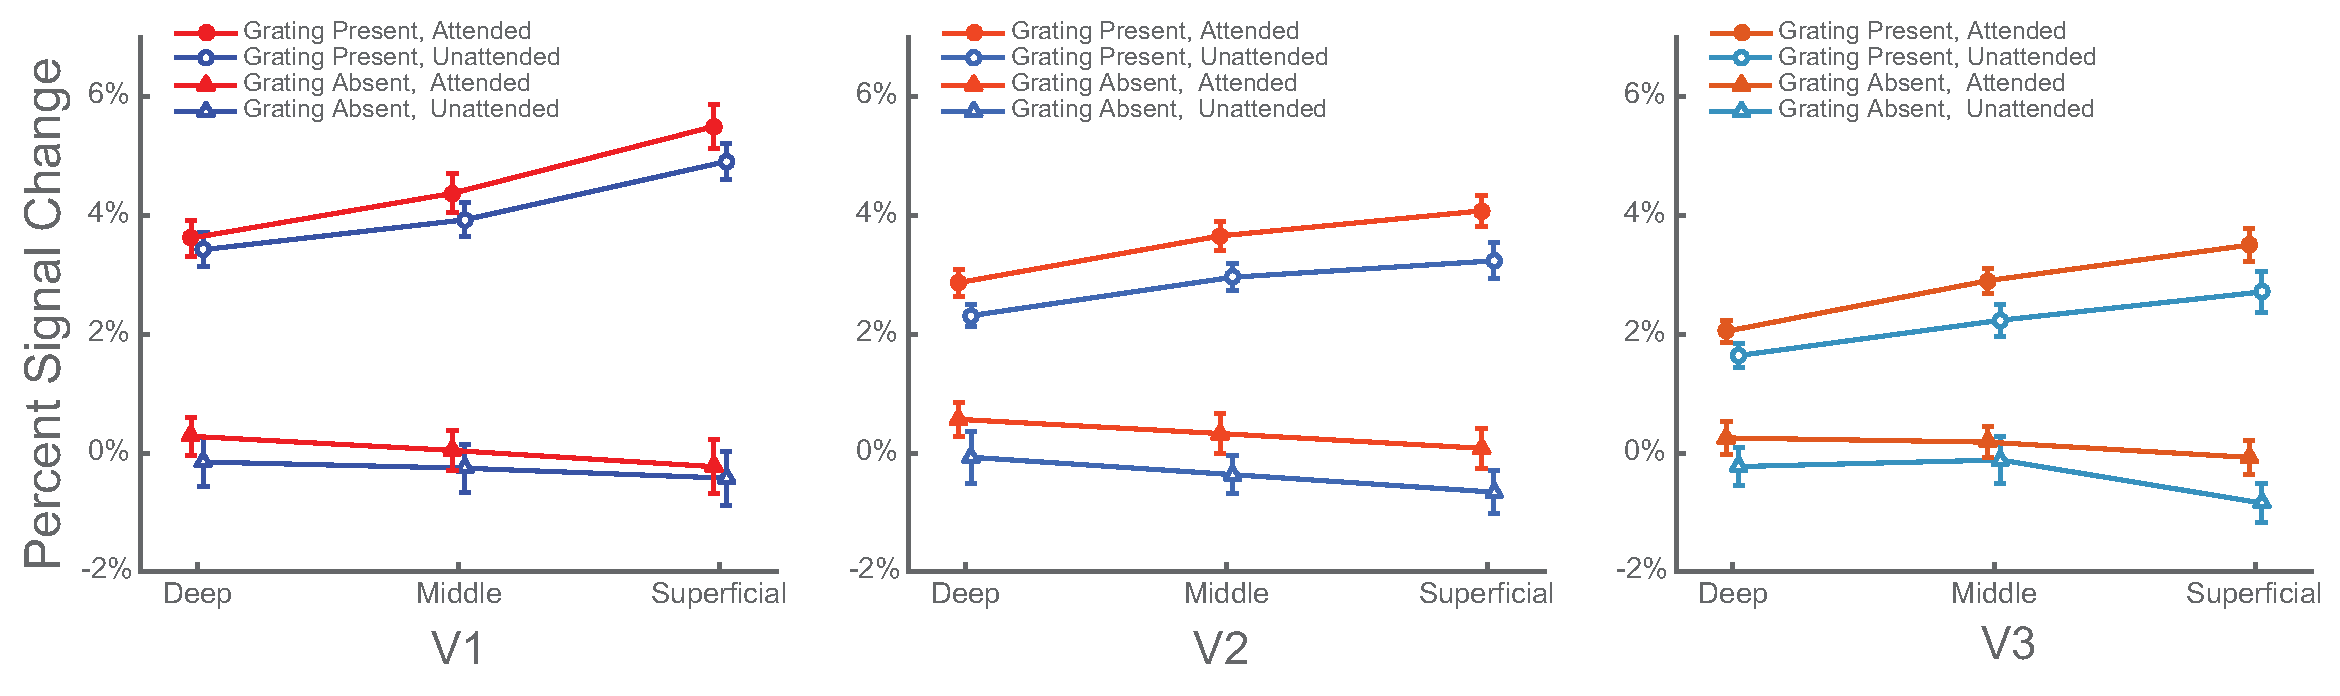
\includegraphics[width=0.8\textwidth, clip=true]{./Chapters/04_Attention/Images/LayerResults}
\caption{Layer-specific amplitude of the BOLD response in the experiment in areas V1-V3. Circles indicate when a grating was presented, squares depict when no grating was presented, at either the attended (red) or unattended (blue) location. When a stimulus was presented, activation reliably increased towards the pial surface. Attention significantly enhanced the BOLD response across all layers. Error bars indicate $\pm$1 SEM.}
\label{fig:layerresults}
\end{figure}



